% !TeX spellcheck = de_DE

\section{Teilprojekt Audioparkour mit CUDA} \label{CUDA_PARKOUR}

Das Teilprojekt Audioparkour mit CUDA stellt ein Anwendungsbeispiel für CUDA in der Signalverarbeitung dar. Der Grundgedanke zur Implementierung dieses Anwendungsfalls ist, ein Eingabesignal in Form einer WAV-Datei mithilfe der Shader Kerne über die CUDA Schnittstelle zu manipulieren, sodass ein Effekt der Positionsveränderung zur gegebenen Soundquelle entsteht. Durch Nutzereingaben können die Positionsdaten in Rotation und Entfernung zum Startpunkt verändert werden. Die Herausforderung ist dabei unter anderem eine Audioquelle zu manipulieren, die gleichzeitig auf einem Wiedergabegerät abgespielt wird. Die Einzelheiten zu diesen Techniken werden im folgendem Kapitel offengelegt.

\subsection{Überblick} \label{sub:manipulator_ov}
In der Ausgangssituation steht die schon im Projekt AudioTracer verwendete WAV-Datei \texttt{2channelKnownFreqTest.wav} zut Verfügung. Analog zum Dateinamen sind zwei Audiokanäle (links und rechts) vorhanden, auf denen jeweils ein harmonisches Audiosignal wiedergegeben wird. Auf dem linken Kanal ist eine Sinuswelle mit einer Frequenz von 300Hz gespeichert. Der rechte Kanal hält eine Sinusfrequenz von 30Hz. Diese Datei bietet sich für Testzwecke an, da auf jedem Kanal nur eine gleichbleibende Frequenz wiedergegeben wird und somit leicht zu unterscheiden ist. 
\begin{figure}[h!]
	\centering      
	\def\svgscale{0.75}
	\includesvg[inkscapelatex=false]{figures/manipulatorOV.svg}
	\caption{Überblick Teilprojekt Audioparkour mit CUDA}
	\label{fig:manipulatorOV}
\end{figure}

In Abbildung \ref{fig:manipulatorOV} ist eine grobe Übersicht auf das Implementierte Audioparkour Projekt zu sehen. Der erste Schritt ist es hier, die WAV-Daten in einer Datenstruktur im erstellten Python Modul verfügbar zu machen. Im Gengensatz zum Projekt AudioTracer liegen die Audiodaten in diesem Fall statisch vor. Es wäre durch leichte Erweiterungen möglich, die beiden Projekte AudioTracer und Audioparkour an dieser Stelle miteinander zu koppeln (dazu mehr im Kapitel \ref{chap:farsight}). Das Python Modul ist für die Initialisierung des CUDA Kontextes und das Verarbeiten der Nutzereingaben zuständig. Außerdem wird die Ausgabe auf einem Audiogerät hier realisiert. Als Nutzereingaben werden Tasten des Pfeiltastenblocks ('up', 'down', 'left', 'right') akzeptiert. Die horizontalen Eingaben verändern eine Rotation und die vertikalen die Entfernung vom Mittelpunkt. 
\begin{figure}[h!]
	\centering      
	\def\svgscale{0.5}
	\includesvg[inkscapelatex=false]{figures/audioParkour.svg}
	\caption{Positionsveränderung Audioparkour}
	\label{fig:audioparkourClock}
\end{figure}

Abbildung \ref{fig:audioparkourClock} zeigt das Grundsätzliche Prinzip der Positionsveränderung in einer Art uhrenförmigen Struktur. Die Positionsangaben sind relativ zum Mittelpunkt dieser \enquote{Uhr} zu betrachten. In dieser Analogie würden die Zeiger in ihrer Rotation und Länge respektive die Position der beiden Lautsprecher bestimmen. Diese Werte werden vom ausführenden Benutzer gesteuert und können während der Wiedergabe der Audiodatei verändert werden. Die Manipulation des Eingabesignals wird passend zum Kontext dieser Arbeit in einem CUDA Kontext realisiert. Bisher wurde die Implementierung der CUDA Schnittstelle für die Programmiersprache C näher erläutert. Da das hier vorgestellte Modul in Python implementiert wurde, sind ein paar Einzelheiten vorher klarzustellen. 

Python hat keine direkte Schnittstelle zur Grafikkarte, kann jedoch Daten vermitteln und wieder extrahieren. Der individuelle auszuführende Code auf den Shader Kernen wird in einem so genannten \texttt{SourceModule} in einem String angegeben. Der String muss eine lauffähige Methode in C mit korrekter Syntax repräsentieren. Diese Methode ist aus der Sektion \ref{sec:audiotracer} bekannten global deklarierte Methode, welche im Host und Device Kontext referenzierbar ist. Das Python Objekt SourceModule gibt eine Referenz zu dieser Methode zurück, welche zu einem späteren Zeitpunkt direkt vom Python Modul ausgeführt werden kann.
Die Wiedergabe eines Audiosignals wird mit dem Paket \texttt{Sounddevice} realisiert. Durch dieses Paket besteht die Möglichkeit, ein Stream Objekt zu erstellen, das die rohen Daten direkt via einer Callback Methode auf einem bestimmten Audiogerät abzuspielen. Die Callback Methode ist die Schlüsselstelle, an der die Manipulation der WAV-Daten eingesetzt werden kann, da ein solcher Audiostream nach der Wiedergabe einer bestimmten Anzahl an Samples - hier Blockgröße genannt - die Callback Methode nach Definition aufruft, damit dort der nächste Block bestimmt werden kann.
Die zwei Techniken der Sound-Manipulation und der Wiedergabe sind dabei nicht abhängig voneinander. Dies ist immens wichtig, da ansonsten in der Zeit, in der der CUDA Teil die Sounddaten manipuliert Verzögerungen in der Wiederhabe zu hören sein könnten. Im schlimmsten Fall würde das Programm hier mit einem Fehler stoppen. Dieses Problem wird dadurch gelöst, dass in der Übergangszeit das zuvor manipulierte Signal wiedergegeben wird, bis die nächste Iteration der CUDA Routine abgeschlossen ist. 

\begin{figure}[hbt!]
	\centering      
	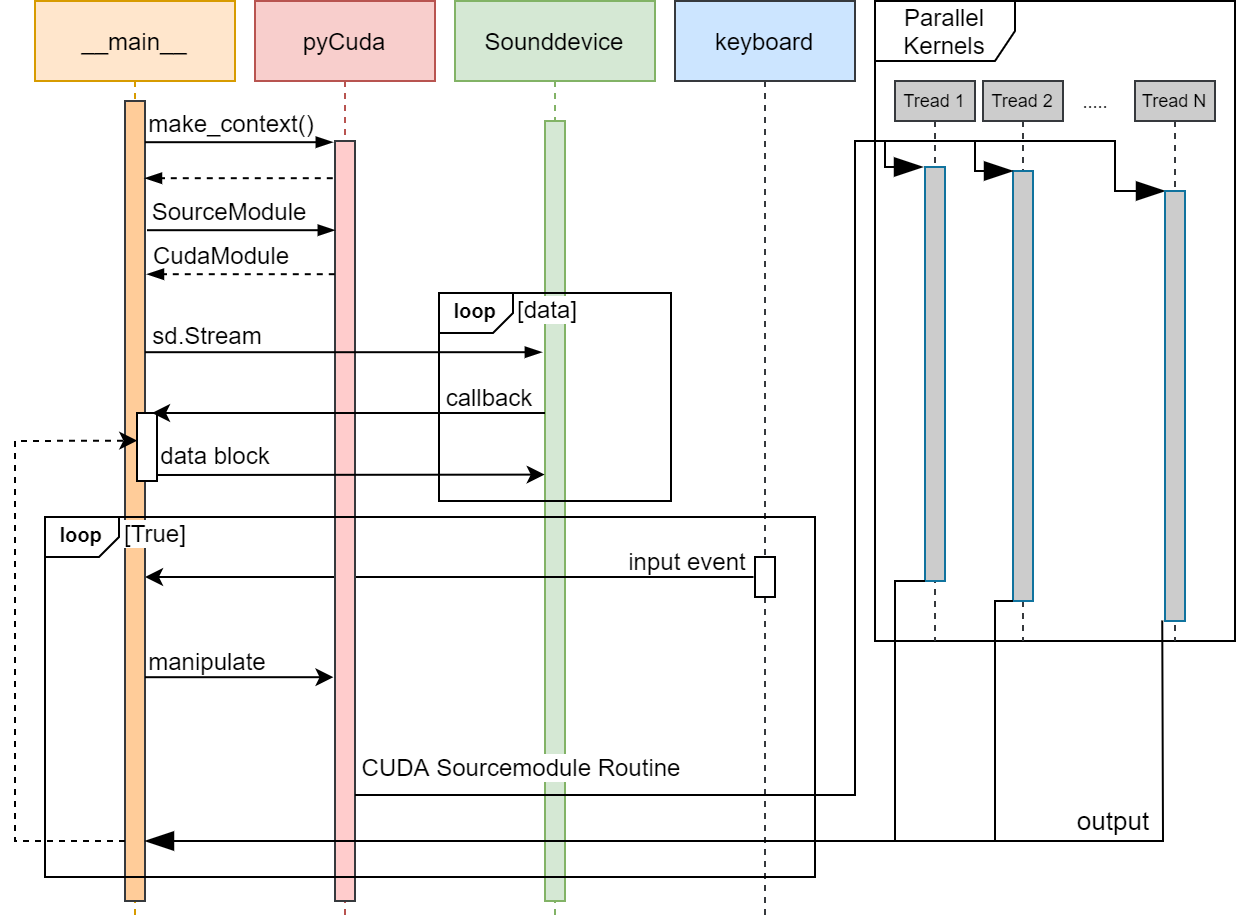
\includegraphics[scale=0.46, angle=-90]{figures/Soundmanipulator_sequence.png}
	\caption{Sequenzdiagramm Audioparkour}
	\label{fig:Seq_soundManipulator}
\end{figure}

\subsection{Code Architektur}

Im folgenden Kapitel werden Einzelheiten zur Implementierung offengelegt. Vor allem die in Sektion \ref{sub:manipulator_ov} beschriebenen Techniken werden hier genauer betrachtet. Zunächst werden die wichtigsten importierten Pakete zur Realisierung des Audioparkour Projekts aufgelistet und deren Funktion im Programm angegeben.

\begin{figure}[h!]
	\lstinputlisting[frame=none, language=C, firstline=1, lastline=8, firstnumber=1 ]{../../Master\_parallel\_fourier\_audio/python/soundManipulator.py}
	\caption{Verwendete Pakete im Projekt Audioparkour}
	\label{fig:audioparkour_packages}
\end{figure}

In Zeile 3 wird das Paket \texttt{scipy.io.wavfile} eingebunden. Dies erlaubt eine leichte Einbindung von WAV-Dateien in das Python Projekt. Im AudioTracer Projekt hat diese Funktionalität die Klasse \texttt{WAVLoader} übernommen. Zeile 4 bindet das wichtigste Paket \texttt{SourceModule} aus dem \texttt{PyCUDA} Projekt ein. Ein SourceModule erlaubt es validen C-Code als Funktion in Python zu verwenden. Wie in Sektion \ref{sub:manipulator_ov} beschrieben wurde, wird diese Schnittstelle benötigt, da es sich bei CUDA um eine C-Library handelt und somit Python nicht nativ unterstützt. Das Paket \texttt{pycuda.driver} aus Zeile 5 ist für die generelle Initialisierung des CUDA Kontextes zuständig und steuert zum Beispiel die Verteilung eines Prozesses auf die CUDA Kernels und die Auswahl der GPU, auf der diese Art von Rechnungen durchgeführt werden sollen. In Zeile 6 wird das Paket \texttt{sounddevice} eingebunden. Darüber wird der Zugriff auf ein Audio Ausgabegerät möglich. Die Nutzereingaben erfolgen über die Tastatur. Die Schnittstelle, um solche Eingaben abzufangen ist das in Zeile 7 eingebundene Paket \texttt{keyboard}. Zeile 8 bindet das Paket \texttt{dataclass} ein. Eine \texttt{dataclass} ist eine in Python interpretierte Klasse oder Struct um z.B. für einen bestimmten Kontext individuelle Attributklassen zu erstellen. 

\begin{figure}[h!]
	\lstinputlisting[frame=none, language=C, firstline=11, lastline=14, firstnumber=11 ]{../../Master\_parallel\_fourier\_audio/python/soundManipulator.py}
	\caption{Python: dataclass}
	\label{fig:audioparkour_dataclass}
\end{figure}

In diesem Fall wird eine \texttt{dataclass} verwendet, um die Positionsdaten zu speichern und für den weiteren Verlauf verfügbar zu machen. Dabei muss die Annotation \texttt{@dataclass} verwendet werden, um built-in Getter- und Setter-Methoden verfügbar zu machen. Zwei Variablen werden analog zur Beschreibung in \ref{sub:manipulator_ov} angelegt. Der Integer Wert \texttt{rotation} gibt die Rotation in eine bestimmte Richtung an. In diesem Projekt wird einem Rotationswert größer dem Wert 0 eine Rotation nach rechts zugeordnet. Analog bildet eine negative Rotation eine Linksdrehung ab. Die float Variable \texttt{distance} gibt die simulierte Distanz zwischen Soundquelle und Hörer an. 
Dies sind die wichtigsten Pakete die benötigt werden, um die beschriebene Funktionalität zu implementieren.

Die nächsten drei Codeblöcke implementieren das Einlesen des WAV-Files, das Erstellen des CUDA Kontexts die Initialisierung von wichtigen später verwendeten Variablen.

\begin{figure}[h!]
	\lstinputlisting[frame=none, language=C, firstline=18, lastline=21, firstnumber=18 ]{../../Master\_parallel\_fourier\_audio/python/soundManipulator.py}
	\caption{Audioparkour: Einlesen der WAV-Datei}
	\label{fig:audioparkour_read_wav_file}
\end{figure}

Im ersten Codestück \ref{fig:audioparkour_read_wav_file} wird in Zeile 18 mithilfe des zuvor eingebundenen Pakets \texttt{scipy.io.wavfile} die Audiodatei eingelesen und als Array Struktur verfügbar. Die Methode \texttt{read} erwartet eine Angabe des Pfades zur WAV-Datei und gibt neben den Kanaldaten die Sample Rate zurück, die im späteren Verlauf verwendet wird. Die Angabe der Anzahl der Audiokanäle muss manuell in der darauffolgenden Zeile durchgeführt werden. Zeile 20 legt eine Kopie des Originalsignals an, auf der die späteren Manipulationen durchgeführt werden. Die Variable \texttt{transitionHelper} ist eine weitere Kopie, die als Überbrückung des asynchronen Vorgangs der Audiomanipulierung Verwendet wird. Mit der Einbindung von CUDA Operationen kann nicht davon ausgegangen werden, dass die aktuell wiedergegebene Audiodatei weiterhin abgespielt werden kann, während sie in Verwendung im CUDA Teil des Programms ist.

\begin{figure}[h!]
	\lstinputlisting[frame=none, language=C, firstline=25, lastline=29, firstnumber=25 ]{../../Master\_parallel\_fourier\_audio/python/soundManipulator.py}
	\caption{Audioparkour: Erstellung des CUDA-Kontext}
	\label{fig:audioparkour_cuda_context}
\end{figure}

Der zweite Codeblock \ref{fig:audioparkour_cuda_context} initialisiert die Verwendung der CUDA Schnittstelle. Dies wird durch die Erstellung eines CUDA Kontexts realisiert. Ein CUDA Kontext ist ein bestimmter Zustand, in der sich die CUDA Runtime API für einen Programmablauf befindet. Dieser Kontext muss konsistent bleiben, beispielsweise ist dieser nur auf dem Thread verfügbar, auf dem er erstellt wurde.
Zeile 25 initialisiert das Device-API-Interface gefolgt von der Auswahl der CUDA-fähigen GPU in Zeile 27. Der CUDA Kontext wird mit der \texttt{make\_context()} der Device API erstellt (Z. 28).

\begin{figure}[h!]
	\lstinputlisting[frame=none, language=C, firstline=31, lastline=35, firstnumber=31 ]{../../Master\_parallel\_fourier\_audio/python/soundManipulator.py}
	\caption{Audioparkour: Globale Variablen}
	\label{fig:audioparkour_globals}
\end{figure}

Im dritten Block der Vorbereitungen zur Implementierung der Wiedergabe- und Manipulationslogik werden wichtige globale Variablen festgelegt. Die Variable \texttt{index} in Zeile 31 wird dafür verwendet, den korrekten Ablauf bei der Wiedergabe der Audiodatei einzuhalten, der via einer Callback Funktion - die im Laufe dieses Kapitels noch aufzuführen ist - bestimmt werden kann. In Zeile 32 wird eine \texttt{block\_size} angegeben. Dies spiegelt die Länge der Audiosamples wieder, die zwischen zwei aufeinander folgenden Callback Funktionsaufrufen wiedergegeben werden und wird zufällig gewählt auf 1024 gesetzt. Die Variable \texttt{blockStream} verhindert, dass die Callback Funktion den gerade manipulierte Datensatz als Soundquelle auswählt. Während des Manipulationsvorgangs wird das zuletzt veränderte Soundsignal wiedergegeben, bis die CUDA Routine erfolgreich beendet wurde. Dies verhindert eine Latenz beim abspielen. Für den Benutzer ist eine so künstlich hergestellte Verzögerung bis der neue Datensatz bereit ist nicht erkennbar. Aus \ref{sec:audiotracer} und \ref{sub:gtx1080} ist bekannt, dass in der Testumgebung eine Geforce GTX 1080 GPU verwendet wurde. Die maximale Anzahl der aktiven Shader Kerne liegt bei 1024 und wird somit in Zeile 34 analog definiert. Zeile 35 initialisiert die zuvor erstellte \texttt{dataclass Position} mit dem Wert 0 für beide Attribute. 

Mit diesen Vorbereitungen können nun die weiteren Implementierungen vorgenommen werden. Es wurde erwähnt, dass seitens CUDA ein so genanntes \texttt{SourceModule} verwendet wurde, um eine Methode in validem C-Code zu erstellen, diese dann in Python zum Aufruf verfügbar wird. 

\begin{figure}[h!]
	\lstinputlisting[frame=none, language=C, firstline=65, lastline=84, firstnumber=65 ]{../../Master\_parallel\_fourier\_audio/python/soundManipulator.py}
	\caption{Audioparkour: SourceModule}
	\label{fig:audioparkour_SourceModule}
\end{figure}

Im abgebildeten Code von Abbildung \ref{fig:audioparkour_SourceModule} wird ein solches SourceModule im konkreten Fall sichtbar. Hier wird die global deklarierte Methode \texttt{manipulate} definiert. Die Signatur dieser Methode ist in Zeile 66 zu sehen. Im Parameter \texttt{int *dest}, hier als Integer Pointer deklariert, werden die manipulierten Sampledaten gespeichert. Der Integer Pointer \texttt{int *src} dient als Datengrundlage und bildet in den einzelnen Durchläufen die Originaldaten in eindimensionaler Form ab. Diese Technik der Abflachung von Arrays wurde bereits im Projekt AudioTracer verwendet, da das Arbeiten mit mehrdimensionalen Arrays generell aufgrund der höheren Komplexität in der Speicherallokation nicht empfohlen wird \cite{nvidia_docs_best_practice}. Der Parameter \texttt{int *rotation} gibt einen Rotationswert im Wertebereich [0, 180[ an. Dieser Wert ist maßgeblich an der Verteilung der Audiosignale auf die anderen Soundkanäle zuständig, denn je nach Rotation werden Teile von benachbarten Kanälen aufaddiert, um einen adäquaten Effekt der Positionsabhängigkeit zu erhalten. Analog bestimmt der Parameter \texttt{float *distance} die simulierte Entfernung zur Soundquelle. Je höher der Wert, desto - einfach ausgedrückt - leiser müssen die einzelnen Soundkanäle werden. Da eine Audiodatei meistens eine höhere Anzahl von Audiosamples aufweist, als CUDA Kernel verfügbar sind, werden alle Audiosamples auf die Kernels aufgeteilt, d.h. jeder CUDA Kern berechnet einen zusammenhängenden Teilbereich für die Ausgabe. Diese Aufteilung wird durch den Parameter \texttt{int *parts} gesteuert. Die Variable \texttt{int *numChannels} wird für die Iteration der einzelnen Audiokanäle benötigt, sowie der Berechnung des Mittels mehrerer addierter Samples, beispielsweise wenn ein Teile eines Channels abhängig von der Rotation in einem anderen zu hören sind.
Auffällig ist hier, dass alle Parameter in Form von Referenzen übergeben werden. Dies war notwendig, da hier ein pass-by-value anders als in offiziellen Dokumentationen \cite{pycuda_docs} nicht möglich ist.

In Zeile 68 wird der Index des Kernelthreads, der eindeutig für jeden ausgeführten Thread verfügbar ist, bestimmt. Dieser wird verwendet, um den \enquote{Zuständigkeitsbereich} eines Threads für die Manipulation zu berechnen. In der darauffolgenden Zeile wird eine Variable \texttt{float modRot} in Abgängigkeit der Rotation geteilt durch den Maximalwert der Rotation bestimmt. Dieser muss bei der Multiplikation mit einem Audiosample zwischen 0 und 1 liegen, da anderenfalls bei größeren Rotationswerten die Wiedergabe an diesen Stellen übersteuern würde.
Zeile 70 beschreibt den Laufbereich einer Schleifeniteration, wobei die zuvor beschriebenen Parameter \texttt{idx} und \texttt{parts} benötigt werden, um geeignete Grenzbereiche zu kalkulieren. Die Iteration wird jeweils um die Anzahl der Audiokanäle erhöht.
Innerhalb dieser Anweisung ist eine weitere Iteration implementiert (Zeile 72-81). Die Hauptaufgabe in diesem Kontext ist die Bestimmung der Ausgabesamples im Array \texttt{dest}. Der aktuelle Sample Index wird dem Integer Feld \texttt{int chIdx} zugewiesen. Das neue Ausgabesample berechnet sich durch die Annahme, dass es sich in diesem Anwendungsfall beispielsweise nach Abbildung \ref{fig:audioparkourClock} um eine menschliche Person positioniert im Mittelpunkt zwischen zwei Audiokanälen handelt. Bei einer Rotation in eine Richtung würde ein Sample, das nur aus dem rechten Audiokanal zu hören ist, zunächst bei fortlaufender Rotation in dieselbe Richtung leiser zu hören sein und Schließlich nur auf dem linken Kanal. Dasselbe muss für die Rückrichtung vom linken auf den rechten Kanal gelten. Nach dieser Analogie würde in Zeile 76f. das aktuell betrachtete Sample mit der Teilrechnung \texttt{src[chIdx] - src[chIdx] * modRot} leiser werden. Dieses wird dann mit einem Anteil des vorherigen Audiokanals addiert \texttt{+src[i + abs(chIdx-1) \% numChannels]}. Dabei wird durch die Verwendung der Methoden \texttt{abs()} und dem Modulo Operator sichergestellt, dass keine Werte außerhalb des Wertebereichs adressiert werden. Wäre der aktuell betrachtete Audiokanal 1 angenommen, würde ein Teil des \texttt{abs(0-1) \% 2 = 1}, also dem zweiten Kanal addiert. Die Addition von Audiokanälen kann so jedoch nicht stehen gelassen werden. Das Ergebnis muss zwingend durch die Anzahl der Kanäle geteilt werden, da die anteiligen Frequenzen sonst nicht mehr stimmen würden. Nach diesem Prinzip werden Reihum alle Audiokanäle manipuliert. Die Berechnung der Distanz ist folgend weniger kompliziert (Z. 79f.). Liegt der Wert der Variable \texttt{distance} nicht zwischen -1 und 1 wird der aktuelle Kanal durch diesem Wert geteilt. Dadurch verändert sich die Amplitude der anteiligen Sinuswellen und es entsteht ein Effekt der Entfernung zum Wiedergabegerät in Form von einer geringeren Lautstärke an der Stelle.

Das hier beschriebene \texttt{SourceModule} wird seitens Python durch die Zuweisung  \texttt{manipulate = mod.get\_function("manipulate")} zugreifbar und kann mit entsprechenden Parametern auf der Grafikkarte ausgeführt werden.

Als nächster Schritt muss ein Audiostream erstellt werden, der zu bestimmten Zeitpunkten verändert werden kann. Das eingebundene Paket Sounddevice bietet eine solche Funktionalität mithilfe der Methode \texttt{Stream(...)} an, deren Einzelheiten im folgenden diskutiert werden.

\begin{figure}[h!]
	\lstinputlisting[frame=none, language=C, firstline=87, lastline=88, firstnumber=87 ]{../../Master\_parallel\_fourier\_audio/python/soundManipulator.py}
	\caption{Audioparkour: Sounddevice Stream}
	\label{fig:audioparkour_sd_stream}
\end{figure}

Die Methode \texttt{Stream} vom Paket sounddevice erwartet im Wesentlichen vier Parameterangaben. Der Parameter \texttt{device} gibt das Ausgabegerät an und wird in diesem Fall mit dem Standardwiedergabegerät \texttt{sd.default.device} beschrieben. Die Sample Rate (\texttt{samplerate}) wurde beim Einlesen des WAV-Files zurückgegeben und in der Variable \texttt{fs\_rate} gespeichert. Die Sample Rate bestimmt, wie viele Samples in einer Sekunde abgespielt werden. Im Parameter \texttt{channels} wird die Anzahl der Audiokanäle an den Audiostream übergeben. Außerdem wird eine Angabe erwartet, um welchen Integer Typ es sich bei den Sampledaten handelt \texttt{dtype}. Der letzte Parameter \texttt{callback} ist im Kontext dieses Projekts ein sehr wichtiger Meilenstein. Es wird eine individuell erstellte Callback-Funktion erwartet, die nach einer bestimmten Menge an wiedergegebenen Samples aufgerufen wird. Diese Menge wird in dem Parameter \texttt{blocksize} gespeichert. Die Callback-Funktion erlaubt es in diesen spezifischen Momenten die aktuelle Wiedergabe zu manipulieren. Die Manipulation muss zwangsweise über die Callback Methode durchgeführt werden, da dadurch gewährleistet wird, dass die korrekte Position der Wiedergabe eingehalten wird. Außerdem würden bei einer direkten Überschreibung des Audiostreambuffers Latenz und Störgeräusche entstehen.

\begin{figure}[h!]
	\lstinputlisting[frame=none, language=C, firstline=38, lastline=39, firstnumber=38 ]{../../Master\_parallel\_fourier\_audio/python/soundManipulator.py}
	
	\lstinputlisting[frame=none, language=C, firstline=46, lastline=49, firstnumber=46 ]{../../Master\_parallel\_fourier\_audio/python/soundManipulator.py}
	
	\lstinputlisting[frame=none, language=C, firstline=52, lastline=62, firstnumber=52 ]{../../Master\_parallel\_fourier\_audio/python/soundManipulator.py}
	
	\caption{Audioparkour: Sounddevice Callback Methode}
	\label{fig:audioparkour_sd_callback}
\end{figure}

Die Callback Methode ist in Abbildung \ref{fig:audioparkour_sd_callback} aufgelistet. Die Methode erwartet die Angabe von fünf Parametern:

\begin{itemize}
	\item \texttt{in\_data}: Dieser Parameter spiegelt die aktuell vom Audiostream verwendeten Audiosamples als Mehrdimensionales Array ab. Hier findet dieser keine Verwendung, da die Wiedergabe zu keinem Callback Zeitpunkt von den Eingabesamples abhängig ist.
	\item \texttt{out\_data}: Dies ist das Ausgabearray. Alle Veränderungen treten ab dem nächsten wiedergegebenem Block in Kraft. Dieser Parameter dient als Ansatzpunkt für die Manipulation der Signaldaten. Der nächste Block der Wiedergabe wird aus dem reorganisierten Ergebnis der CUDA Ausgabe aus \ref{fig:audioparkour_SourceModule} bestimmt. Die CUDA Ausgabe muss dafür vor dem Callback in einer passenden Array Struktur vorliegen. 
	\item \texttt{frames}: Der Parameter \texttt{frames} gibt die Anzahl der Samples an, die zwischen dem aktuellen und vorherigen Callback wiedergegeben wurden. Dies findet in diesem Anwendungsfall keine Relevanz.
	\item \texttt{time} ist ein Objekt, das Timestamps über die Signalumwandlung von digital zu analog und analog zu digital für jeweils das erste Sample in in- und output Buffer.
	\item \texttt{status}: Gibt Fehler Flags zurück, wenn ein Buffer Über- oder Unterlauf während der Wiedergabe festgestellt wird. Fehler werden in diesem Fall lediglich ausgegeben, treten in der Regel allerdings nicht auf.
\end{itemize}

In Zeile 39 der Callback Methode werden die zuvor angelegten globalen Variablen auch als solche deklariert. Python Variablen sind Scope gebunden, sodass ohne diese Deklaration die beiden Variablen \texttt{index} und \texttt{blockStream} im äußeren Scope unverändert bleiben würden. Erstere kann so in Zeile 62 korrekt inkrementiert werden. Zeile 46f. bewirkt, dass die Wiedergabe in einer Schleife abgespielt wird. Dies wurde als hilfreich befunden, um auch mit kürzeren Audiodateien zu arbeiten, deren Wiedergabe schnell beendet wird, ohne eine Möglichkeit für viele Nutzereingaben zu gewährleisten. 
In Zeilen 49 bis 53 wird die Länge des nächste Output Buffers evaluiert und erhält initial den Wert der globalen \texttt{block\_size}. Es kann sein, dass die Länge des letzten Blocks im Audiostream kleiner ist als block\_size. Für diesen Fall wird die entsprechende Differenz kalkuliert. 
Die Bestimmung der Samples des nächsten Blocks wird innerhalb der Zeilen 55 bis 59 durchgeführt. Prinzipiell wird das Ausgabearray in Form des Ausgabearrays mit Nullen gefüllt. Danach werden die neuen Samples kopiert. Die Bool'sche Variable \texttt{blockStream} wird verwendet um die eingangs erwähnte Problemstellung zu kompensieren, dass während der CUDA Kontext aktiv Veränderungen am Audiosignal vornimmt, dieses nicht gleichzeitig als Input benutzt werden kann. In dieser Übergangszeit wird die aktuelle Wiedergabe zur Überbrückung fortgesetzt. Zuletzt werden die Sampledaten in das Ausgabe Array \underline{kopiert}. 


An diesem Punkt ist der Audiostream etabliert, das SourceModule interpretiert und alle restlichen Vorarbeiten getroffen, um die Nutzereingaben und die damit verbundene CUDA Routine in einer wiederkehrenden Schleifenoperation abzuarbeiten. 

\begin{figure}[h!]
	\lstinputlisting[frame=none, language=C, firstline=91, lastline=101, firstnumber=91 ]{../../Master\_parallel\_fourier\_audio/python/soundManipulator.py}
	\caption{Audioparkour: Nutzereingaben}
	\label{fig:audioparkour_userInput}
\end{figure}

Nutzereingaben können über die Pfeiltasten getätigt werden. Die Methode \texttt{is\_pressed} wird dabei verwendet, um zu überprüfen, ob ein jeweiliger Tastenanschlag getätigt wurde. Werden die Pfeiltasten links und rechts betätigt wird die Rotation um jeweils die Zahl 1 dekrementiert bzw. inkrementiert. Anschließend wird der Modulo Operator verwendet, damit die Rotation den Wert 180 nicht überschreiten. Im Prinzip kann hier eine Angabe in Grad angenommen werden.
Bei Vertikalen Pfeiltasteneingaben wird die Distanz de- bzw. inkrementiert. 
Sonstige Eingaben werden nicht unterstützt.

Erfolgt eine gültige Nutzereingabe, wird der hintere Teil \ref{fig:audioparkour_cuda+arrayShaping} der while Schleife ausgeführt, der vor allem die CUDA Methode \texttt{manipulate} aufruft, die über das SourceModule Konstrukt erstellt wurde. Die Eingabeparameter müssen mit dem Präfix \texttt{drv.In} versehen werden. Dies löst eine korrekte Speicherreservierung auf der GPU aus. Analog wird die Ausgabe im Python Kontext durch den Präfix \texttt{drv.Out} nach dem Abschluss der CUDA Routine zugreifbar. Außerdem müssen Integer und Float Variablen in die entsprechenden C-Typen umgewandelt werden. Die Blockdimensionen werden nicht weiter auf mehrere Dimensionen aufgeteilt. Dies ist an dieser Stelle nicht nötig, da nur der Index des Threads für diesen Anwendungsfall benutzt wird (Zeile 111 - 114). In Zeilen 105 wird das zuletzt verwendete Signal in das Übergangsarray \texttt{transitionHelper} kopiert. In Verbindung mit der Variable \texttt{blockStream} wird dieses Signal ab hier wiedergegeben, bis die CUDA Operationen abgeschlossen wurden. Das Originalsignal wird in Zeile 107 zu einem eindimensionalen Array und in den passenden Datentyp dabei konvertiert. Nach der Manipulation müss diese Dimensionen wiederhergestellt werden (Zeile 116). Das Ausgabearray wird zunächst mit dem Wert 0 gefüllt, um die Struktur der Eingabe beizubehalten. \texttt{parts} gibt die Anzahl der Teilstücke an, die Jeder CUDA Kernel bearbeiten muss. 

\begin{figure}[h!]
	\lstinputlisting[frame=none, language=C, firstline=105, lastline=116, firstnumber=105 ]{../../Master\_parallel\_fourier\_audio/python/soundManipulator.py}
	\caption{Audioparkour: Manipulation über CUDA}
	\label{fig:audioparkour_cuda+arrayShaping}
\end{figure}

In diesem Python Quellcode des AudioParkour Projekts greifen verschiedene Faktoren ineinander mit teilweise asynchron laufenden Callback Methoden und einem CUDA Kontext der parallel Daten manipuliert, die im Callback verwendet werden. Diese Faktoren bringen eine nicht zu unterschlagene Komplexität mit sich, da viele logische Sprünge notwendig sind.